\documentclass{article}
\usepackage[utf8]{inputenc}
\usepackage{tkz-graph} % http://mirrors.ibiblio.org/CTAN/graphics/pgf/contrib/tikz-network/tikz-network.pdf

\title{Exact and heuristic approaches to prize collecting tour construction (working title)}

\author{Clara Martins, Daniel Monteiro, Gonçalo Pascoal, Rosaldo Rossetti \\
\normalsize \texttt{\{up201806528, up201806185, up201806332, rossetti\}@fe.up.pt}}

\date{April 2020}

\begin{document}

\maketitle

\begin{abstract}
This is a simple paragraph at the beginning of the 
document. A brief introduction about the main subject.

Sightseeing can be hard without a path or someone to help. So, the [app name] is here to calculate the best, most efficient and less expensive route for you to go sightseeing around the city or the country.
\end{abstract}

\section{Introduction}

\subsection{Case study: A sightseeing tour planning app}
% A apresentação do problema
We were presented with the following problem: to create a tourist app capable of creating the most enjoyable tour for the user.

Given the maximum time to do the tour, a start and a destination, we wish to find the best touristic tour that contains the biggest amount of points of interest suitable to the user.

The tours and the kinds of points of interest visited may vary according to the user's preferences, the amount of available time and the kind of transportation used. The visited points of interest ought to match the user's preferences.

\section{Reduction to a graph problem}

A street map with all the points of interest (POIs) can be converted to a weighted directed graph. The POIs can then be a subset of the graph's vertices with a specific prize assigned to each of them. This prize would depend on the user's preferences (for example, if a user wishes to prioritise historical landmarks, their respective vertices' prizes may be inflated). The start and finish are also vertices in the graph. 

\section{Formalization of the problem}

\noindent
Inputs:
\begin{itemize}
    \item A graph $G = (V, E)$ with non-negative directed edges
    \item A set of POI vertices $P$ such that $P \subseteq V$\footnote{In a practical implementation, $P$ and $f$ should be replaced with an associative array}
    \item A function $f$ that maps a POI vertex $v \in P$ to a score (such that $f(v_{i}) = s_{i}$)
    \item Start $S$ and finish $F$ vertices such that $S, F \in V$
    \item A budget $B$
\end{itemize}

\noindent
Output:
\begin{itemize}
    \item A list of vertices (a path) that maximizes the total score (the sum of the scores of the POI vertices in the list) and verifies the following conditions:
    \begin{enumerate}
        \item It begins in $S$ and finishes in $F$
        \item The total cost of the path (sum of the edges' weights) isn't greater than $B$
    \end{enumerate} 
\end{itemize}

\noindent
Decision Variables:
\begin{itemize}
    \item Origin
    \item Destination
    \item Transportation Method
    \item Time Available
    \item Budget Available
\end{itemize}

\noindent
Objective Function:
\begin{itemize}
    \item Objective Function (???)
    \begin{enumerate}
        \item Maximize $g = \sum f(v_i)$
        \item Minimize $h = \sum weight(v_i, v_{i+1})$
    \end{enumerate}
\end{itemize}

\noindent
Constraints:
\begin{itemize}
    \item There must exist at least one list of vertices (a path) that begins in $S$, finishes in $F$ and whose total cost is lower than $B$
\end{itemize}


\section{Overview of the problem and the reduction process}

\subsection{An instance of the problem}

Lets begin with a graph $G = (V, E)$:
\begin{center}
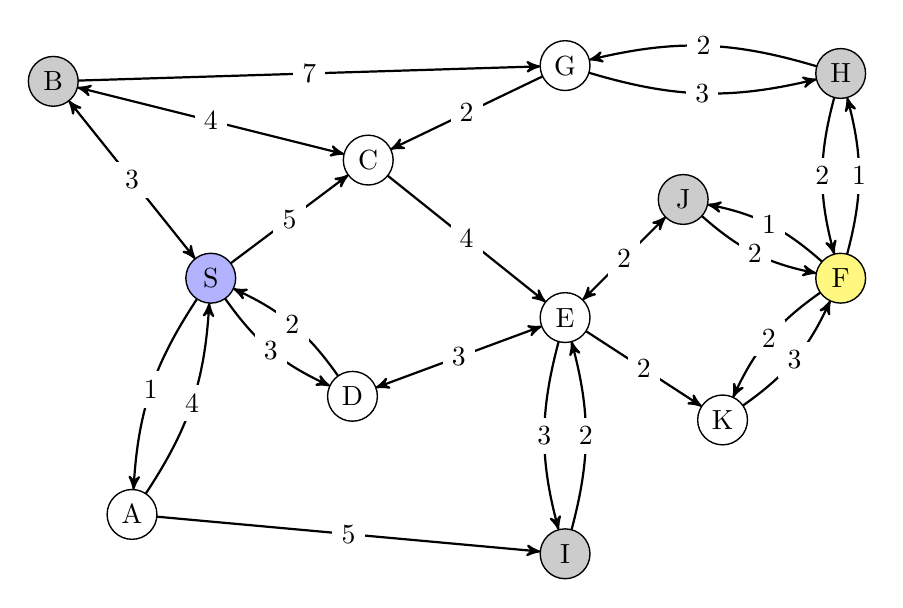
\begin{tikzpicture}
    \Vertex[x=0,   y=0]   {A}
    \Vertex[x=3,   y=4.5] {C}
    \Vertex[x=2.8, y=1.5] {D}
    \Vertex[x=5.5, y=2.5] {E}
    \Vertex[x=5.5, y=5.7] {G}
    \Vertex[x=7.5, y=1.2] {K}
   
    \tikzset{VertexStyle/.append  style={fill = black!20}}
    \Vertex[x=-1,  y=5.5]  {B}
    \Vertex[x=9,   y=5.6]  {H}
    \Vertex[x=5.5, y=-0.5] {I}
    \Vertex[x=7,   y=4]    {J}
   
    \tikzset{VertexStyle/.append  style={fill = blue!30}}
    \Vertex[x=1, y=3] {S}
    \tikzset{VertexStyle/.append  style={fill = yellow!50}}
    \Vertex[x=9, y=3] {F}
    
    \tikzset{EdgeStyle/.style={<->, >=stealth'}}
    \Edge[label=$4$](B)(C)
    \Edge[label=$3$](B)(S)
    \Edge[label=$2$](E)(J)
    \Edge[label=$3$](D)(E)
    
    \tikzset{EdgeStyle/.style={->, >=stealth'}}
    \Edge[label=$5$](A)(I)
    \Edge[label=$7$](B)(G)
    \Edge[label=$5$](S)(C)
    \Edge[label=$2$](G)(C)
    \Edge[label=$2$](E)(K)
    \Edge[label=$4$](C)(E)

    \tikzset{EdgeStyle/.style={->, bend right=15, >=stealth'}}
    
    \Edge[label=$1$](S)(A)
    \Edge[label=$4$](A)(S)
    
    \Edge[label=$3$](S)(D)
    \Edge[label=$2$](D)(S)
    
    \Edge[label=$3$](E)(I)
    \Edge[label=$2$](I)(E)
    
    \Edge[label=$3$](K)(F)
    \Edge[label=$2$](F)(K)
    
    \Edge[label=$2$](J)(F)
    \Edge[label=$1$](F)(J)
    
    \Edge[label=$2$](H)(F)
    \Edge[label=$1$](F)(H)
    
    \Edge[label=$3$](G)(H)
    \Edge[label=$2$](H)(G)

\end{tikzpicture}

For the sake of the reader, we color-coded the vertices: the starting vertex is in blue, the destination vertex is in yellow, and the POI vertices are in grey.
\end{center}

\noindent
The remaining input arguments are as follows:
\begin{itemize}
    \item $P= \{$B, H, I, J$\}$
    \item The function $f$ can be defined as follows:
    \begin{itemize}
        \item $f($B$)=1$
        \item $f($H$)=2$
        \item $f($I$)=3$
        \item $f($J$)=4$
    \end{itemize}
    \item $S=$ S
    \item $F=$ F
    \item $B=12$
\end{itemize}

\subsection{Verifying that a solution exists}
The first step towards finding a solution a verifying that a solution exists at all. This can be done in this specific problem by verifying that a path with a cost no greater than $B$ exists:
\begin{center}
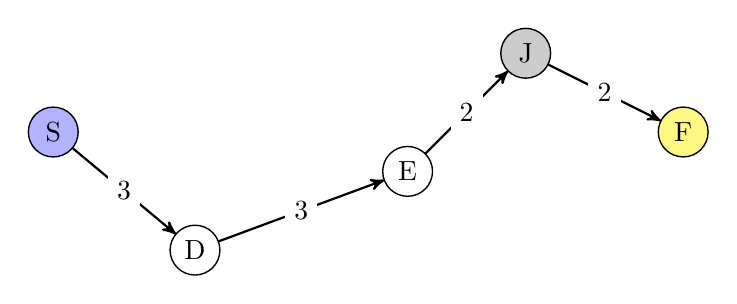
\begin{tikzpicture}
    \Vertex[x=2.8, y=1.5] {D}
    \Vertex[x=5.5, y=2.5] {E}

    \tikzset{VertexStyle/.append  style={fill = black!20}}
    \Vertex[x=7,   y=4]    {J}
   
    \tikzset{VertexStyle/.append  style={fill = blue!30}}
    \Vertex[x=1, y=3] {S}
    \tikzset{VertexStyle/.append  style={fill = yellow!50}}
    \Vertex[x=9, y=3] {F}
    
    \tikzset{EdgeStyle/.style={->, >=stealth'}}
    \Edge[label=$2$](E)(J)
    \Edge[label=$3$](D)(E)
    \Edge[label=$3$](S)(D)
    \Edge[label=$2$](J)(F)
\end{tikzpicture}

S $\rightarrow$ D $\rightarrow$ E $\rightarrow$ J $\rightarrow$ S
\end{center}

The cost of this path is $10$, which is not greater than $B$. Therefore, a solution exists.

\subsection{The solution}
Given these inputs, the path (list of vertices) that maximizes the score is
\begin{center}
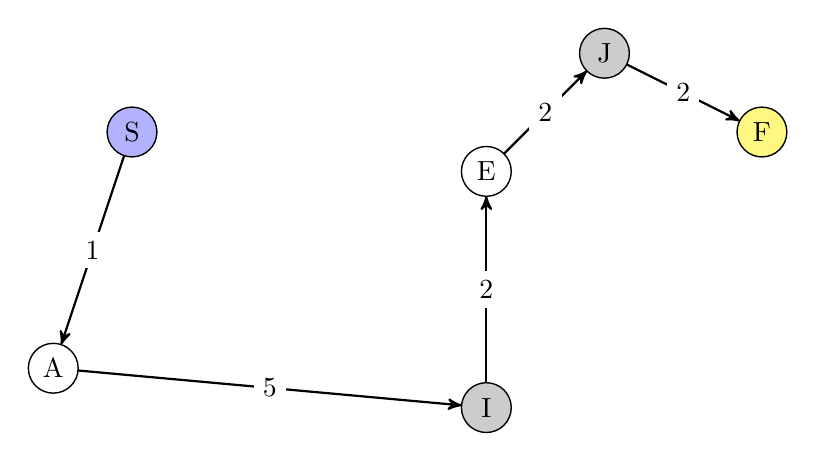
\begin{tikzpicture}
    \Vertex[x=0,   y=0]   {A}
    \Vertex[x=5.5, y=2.5] {E}

    \tikzset{VertexStyle/.append  style={fill = black!20}}
    \Vertex[x=5.5, y=-0.5] {I}
    \Vertex[x=7,   y=4]    {J}
   
    \tikzset{VertexStyle/.append  style={fill = blue!30}}
    \Vertex[x=1, y=3] {S}
    \tikzset{VertexStyle/.append  style={fill = yellow!50}}
    \Vertex[x=9, y=3] {F}
    
    \tikzset{EdgeStyle/.style={->, >=stealth'}}
    \Edge[label=$2$](E)(J)
    \Edge[label=$5$](A)(I)
    \Edge[label=$1$](S)(A)
    \Edge[label=$2$](I)(E)
    \Edge[label=$2$](J)(F)
\end{tikzpicture}

S $\rightarrow$ A $\rightarrow$ I $\rightarrow$ E $\rightarrow$ J $\rightarrow$ F
\end{center}

The cost of this path is $12$, which is not greater than $B$. The total score can be obtained by taking all of the POI vertices in the path and summing their scores: $f($I$) + f($J$) = 3 + 4 = 7$.

\subsection{Key insights}
Given that the total score function only depends on the POI vertices in the path, the graph can be modified, as long as:
\begin{enumerate}
    \item $S$, $F$ and the POI nodes remain in the graph
    \item The cost of the shortest paths from $S$ to $F$ and the POI vertices, from the POI vertices to $F$, and between all the POI vertices remain the same
\end{enumerate}

Taking these restrictions into account, we can modify the solution path without invalidating it:
\begin{center}
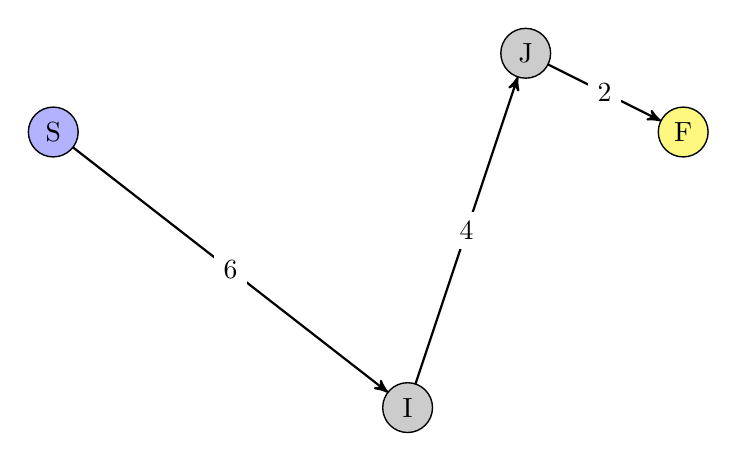
\begin{tikzpicture}
    \tikzset{VertexStyle/.append  style={fill = black!20}}
    \Vertex[x=5.5, y=-0.5] {I}
    \Vertex[x=7,   y=4]    {J}
   
    \tikzset{VertexStyle/.append  style={fill = blue!30}}
    \Vertex[x=1, y=3] {S}
    \tikzset{VertexStyle/.append  style={fill = yellow!50}}
    \Vertex[x=9, y=3] {F}
    
    \tikzset{EdgeStyle/.style={->, >=stealth'}}
    \Edge[label=$6$](S)(I)
    \Edge[label=$4$](I)(J)
    \Edge[label=$2$](J)(F)
\end{tikzpicture}

S $\rightarrow$ I $\rightarrow$ J $\rightarrow$ F
\end{center}

As predicted, the cost of this path is $12$ and the total score is $7$.

\subsection{Reducing the graph to a fully connected directed graph}
We can take advantage of this malleability of the graph by removing all the nodes that aren't $S$, $F$, or a POI vertex, therefore decreasing its size considerably. This can be done by calculating cost of the shortest paths from $S$ to $F$ and the POI vertices, from the POI vertices to $F$, and between all the POI vertices.
\begin{center}
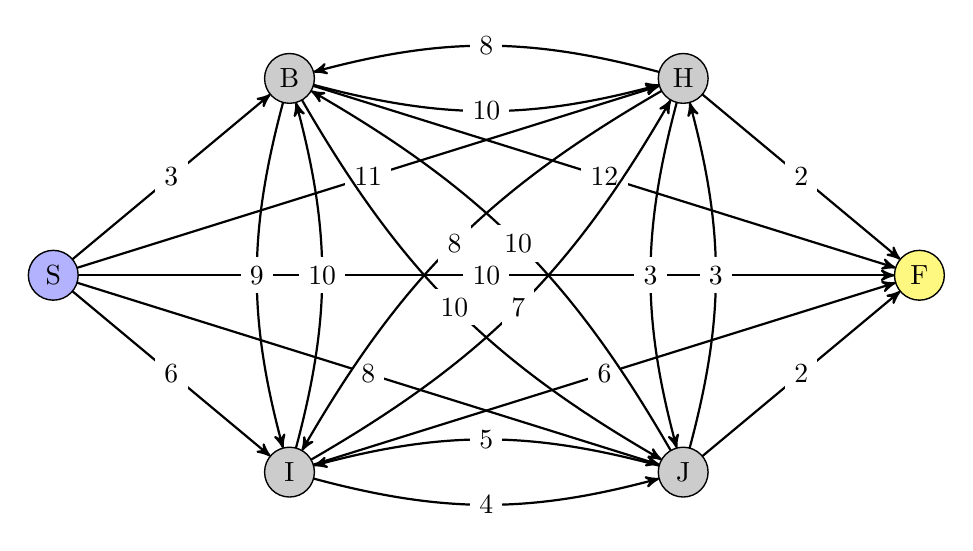
\begin{tikzpicture}
    \tikzset{VertexStyle/.append  style={fill = black!20}}
    \Vertex[x=3, y=5] {B}
    \Vertex[x=8, y=5] {H}
    \Vertex[x=3, y=0] {I}
    \Vertex[x=8, y=0] {J}
   
    \tikzset{VertexStyle/.append  style={fill = blue!30}}
    \Vertex[x=0, y=2.5] {S}
    \tikzset{VertexStyle/.append  style={fill = yellow!50}}
    \Vertex[x=11, y=2.5] {F}
    
    \tikzset{EdgeStyle/.style={->, >=stealth'}}
    \Edge[label=$10$](S)(F)
    
    \Edge[label=$3$](S)(B)
    \Edge[label=$11$](S)(H)
    \Edge[label=$6$](S)(I)
    \Edge[label=$8$](S)(J)
    
    \Edge[label=$12$](B)(F)
    \Edge[label=$2$](H)(F)
    \Edge[label=$6$](I)(F)
    \Edge[label=$2$](J)(F)
    
    \tikzset{EdgeStyle/.style={->, bend right=15, >=stealth'}}
    \Edge[label=$10$](B)(H)
    \Edge[label=$9$](B)(I)
    \Edge[label=$10$](B)(J)
    
    \Edge[label=$10$](I)(B)
    \Edge[label=$4$](I)(J)
    \Edge[label=$7$](I)(H)
    
    \Edge[label=$10$](J)(B)
    \Edge[label=$5$](J)(I)
    \Edge[label=$3$](J)(H)

    \Edge[label=$8$](H)(B)
    \Edge[label=$8$](H)(I)
    \Edge[label=$3$](H)(J)
\end{tikzpicture}
\end{center}

We would like to point out that the solution's path cost and total score remains unaltered. However, the paths between every vertex of this solution path would need to be recomputed in order to recover the original solution path.
\begin{center}
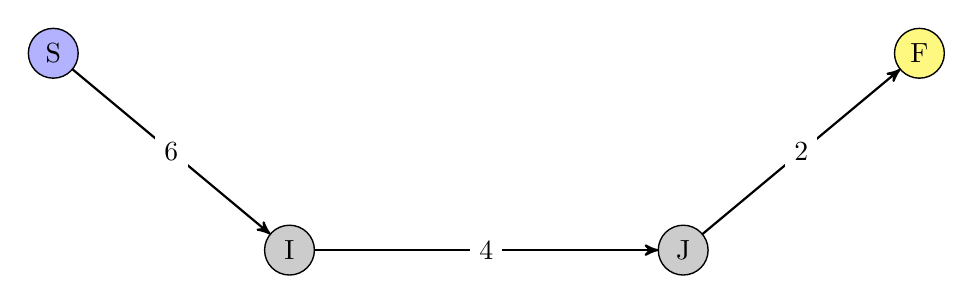
\begin{tikzpicture}
    \tikzset{VertexStyle/.append  style={fill = black!20}}
    \Vertex[x=3, y=0] {I}
    \Vertex[x=8, y=0] {J}
   
    \tikzset{VertexStyle/.append  style={fill = blue!30}}
    \Vertex[x=0, y=2.5] {S}
    \tikzset{VertexStyle/.append  style={fill = yellow!50}}
    \Vertex[x=11, y=2.5] {F}
    
    \tikzset{EdgeStyle/.style={->, >=stealth'}}
    \Edge[label=$6$](S)(I)
    \Edge[label=$2$](J)(F)
    \Edge[label=$4$](I)(J)
\end{tikzpicture}

S $\rightarrow$ I $\rightarrow$ J $\rightarrow$ F

The solution's path cost and total score remains unaltered.
\end{center}

The final modification that needs to be done to convert this graph to a fully connected directed graph, is to "merge" S and F, by redirecting the edges that previously went to F, to S. However, this violates condition 1 from subsection 4.4 (S,F and the POI vertices must be preserved). In order to perform this final modification, additional restrictions must be set:
\begin{enumerate}
    \item The existence of a path beginning in S and finishing in F cost is lower than $B$ must be asserted beforehand
    \item When reconstructing the original path, F has to be appended to the end of the path
\end{enumerate}

Taking these new constraints into account, we can perform our final modification.

\begin{center}
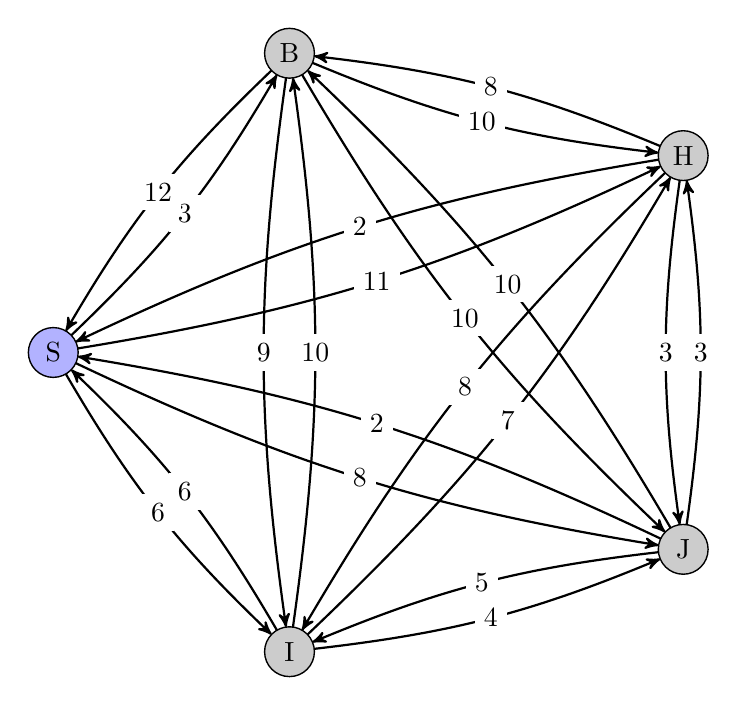
\begin{tikzpicture}
    \tikzset{VertexStyle/.append  style={fill = black!20}}
    \Vertex[x=3, y=6.3] {B}
    \Vertex[x=8, y=5] {H}
    \Vertex[x=3, y=-1.3] {I}
    \Vertex[x=8, y=0] {J}
   
    \tikzset{VertexStyle/.append  style={fill = blue!30}}
    \Vertex[x=0, y=2.5] {S}
    
    \tikzset{EdgeStyle/.style={->, bend right=8, >=stealth'}}

    \Edge[label=$3$](S)(B)
    \Edge[label=$11$](S)(H)
    \Edge[label=$6$](S)(I)
    \Edge[label=$8$](S)(J)
    
    \Edge[label=$12$](B)(S)
    \Edge[label=$2$](H)(S)
    \Edge[label=$6$](I)(S)
    \Edge[label=$2$](J)(S)
    
    \Edge[label=$10$](B)(H)
    \Edge[label=$9$](B)(I)
    \Edge[label=$10$](B)(J)
    
    \Edge[label=$10$](I)(B)
    \Edge[label=$4$](I)(J)
    \Edge[label=$7$](I)(H)
    
    \Edge[label=$10$](J)(B)
    \Edge[label=$5$](J)(I)
    \Edge[label=$3$](J)(H)

    \Edge[label=$8$](H)(B)
    \Edge[label=$8$](H)(I)
    \Edge[label=$3$](H)(J)
\end{tikzpicture}
\end{center}

TODO: Agora o path é um ciclo, reduzimos o problema a uma instância de ACCTSP, e o grafo pode ser  representado por uma matriz, isto permite-nos dividir o problema em duas partes: redução e TSP

\end{document}